\chapter{EXPERIMENTAL OPTIMIZATION OF PLASMA-LIQUID INTERACTIONS: VHF SOURCE}
\label{chap:expt_opt}

\Cref{chap:basic_science} outlines fundamental modeling efforts aimed at describing the physical and chemical phenomena that occur in plasma-liquid systems. \Cref{chap:zapdos} outlines the tool we created in order to better conduct our modeling efforts. To date modeling has been used to gain a better qualitative understanding of transport processes in convective plasma-liquid systems (\cref{sec:plasfree_model}) and to explore the effects of key interfacial parameters on plasma properties (\cref{sec:plasliq}). Model geometries have been based on relatively simple experimental set-ups (point-to-plane corona discharge for \cref{sec:plasfree_model}) or simplified to one dimension as in \cref{sec:plasliq}. However, the groundwork has been laid to model more complex plasma-liquid geometries and exotic electromagnetic fields. Such models will be used to describe the physiochemical properties observed in the complex experimental configurations described in this chapter. This chapter outlines plasma-liquid geometries that exhibit increasing degrees of plasma-liquid contact. In \cref{sec:base} we describe our base experimental configuration: a very high frequency (VHF) atmospheric plasma source that is pointed down into a reservoir of water such that the end of the plasma column is in direct contact with the water surface. In \cref{sec:spray} we discuss spraying water droplets directly through the plasma. After discussing the typical electrodes used on the VHF source in \cref{sec:electrodes}, we introduce in \cref{sec:water_electrodes} a completely novel design where the VHF source is pointed upward and water is pumped through the center of the inner conductor to form a water layer on top of the powered electrode. Finally, in \cref{sec:aq_chem} we show experimental measurements of aqueous chemistry generated by our plasma-liquid systems. We hope to reproduce our experimental measurements in \cref{sec:aq_chem} using a future combination and extension of the models and code described in \cref{chap:basic_science,chap:zapdos}.

\section{Base Set-up}
\label{sec:base}

The experimental set-up shown in \cref{fig:batch_scheme} is known as the ``batch'' set-up. It was the first plasma-water configuration explored by the group. Originally it was intended for degradation of perfluorinated compounds like perfluorooctanesulfonic acid (PFOS) and perfluorootanoic acid (PFOA). It turned out that the batch configuration was unable to degrade these persistent chemicals; however, in the process it was discovered that the configuration generated large amounts of NO$_x$, mostly NO$_3^-$, in the aqueous phase. Generation of nitrogen and oxygen species (RONS) in solution by plasmas is now a well-known phenomenon in the plasma-liquid community; however, at the time it was a novel discovery for our group. Recognizing that aqueous nitrogen, specifically NO$_3^-$, is a key component in fertilizer, we were motivated to begin a study in collaboration with the horticulture department of plant fertilization using plasma activated water (PAW). This study is outlined in \cref{sec:fertigation}. Later, the batch configuration was used in exploration of dioxane degradation; this is discussed in \cref{sec:dioxane}.

Depending on the application, delivered power to the plasma for the batch configuration ranges between 350 and 1000 W. Many different gases are used, including air, argon, helium, nitrogen, and carbon dioxide. Gas flow rates range from 2-5 standard cubic feet per minute. The gap distance between the powered electrode and the water surface range from a few milimeters to a couple centimeters, with larger gap distances typically used in combination with larger gas flow rates in order to avoid splashing of the electrode and extinguishing of the plasma. Water treatment volumes typically span 100-500 mL for persistent chemical studies up to several liters for PAW generation in the fertigation experiments.

\begin{figure}[htbp]
  \centering
  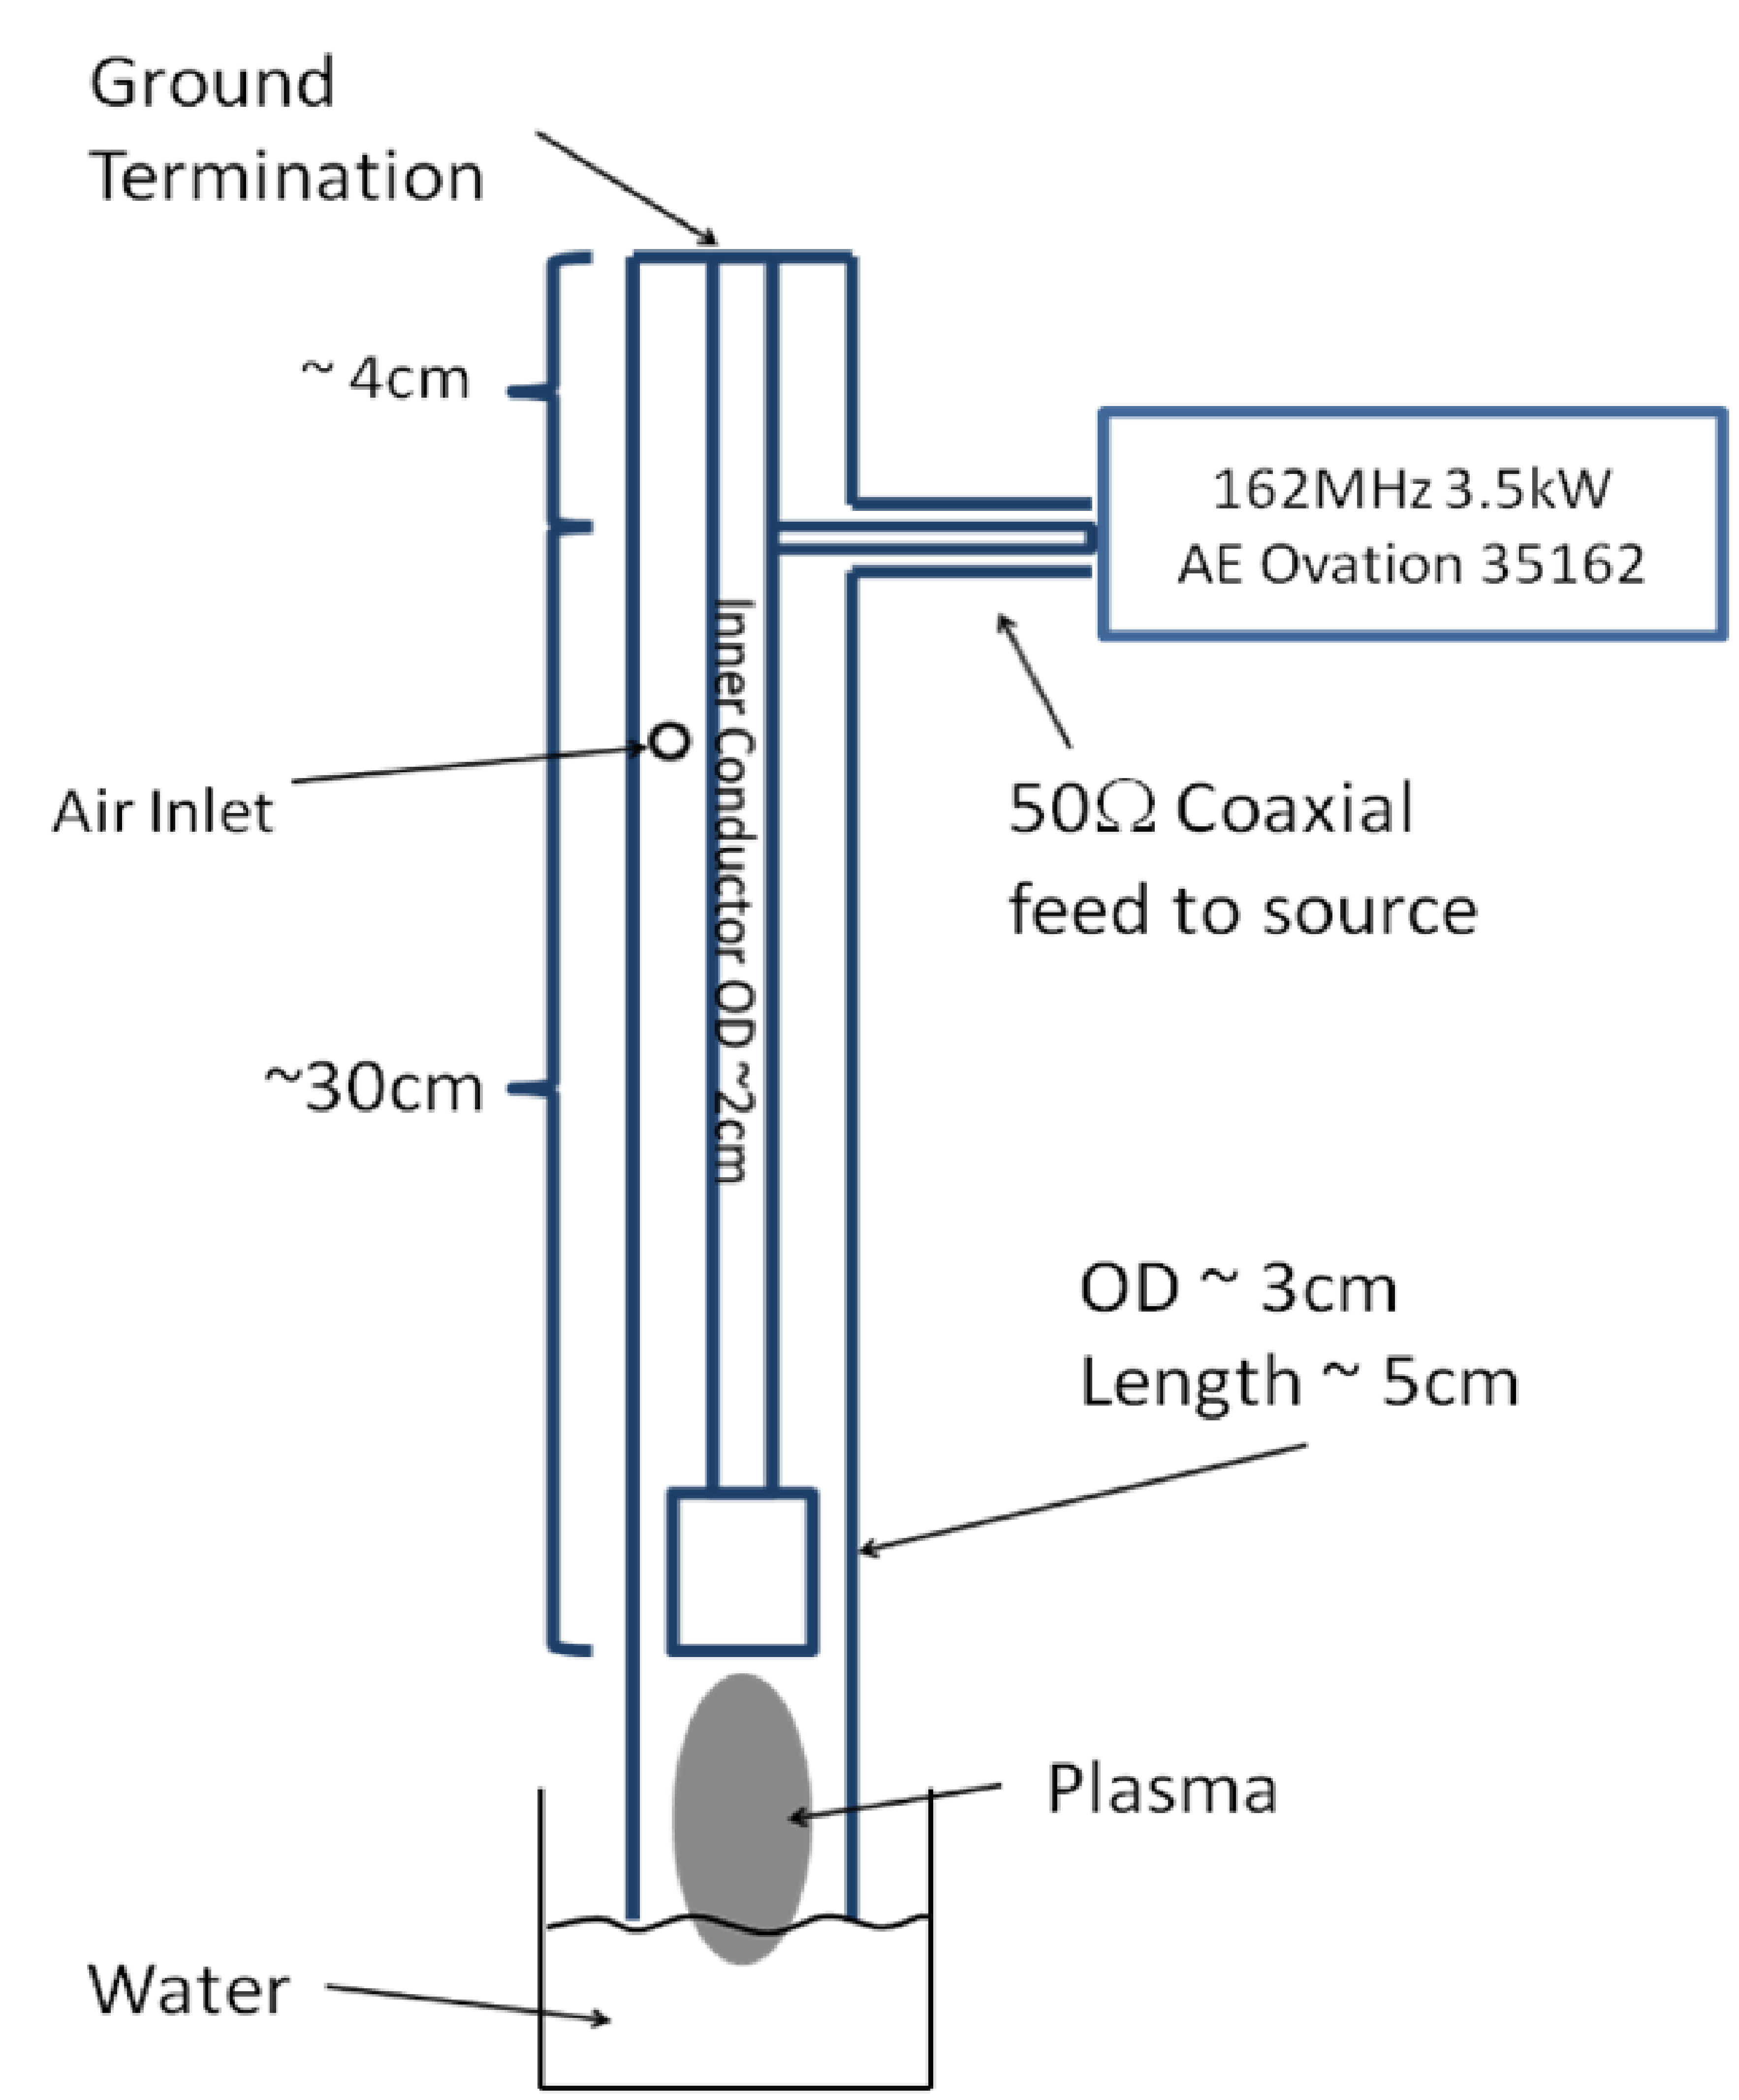
\includegraphics[width=0.9\textwidth]{Figure1_word.pdf}
  \caption{Schematic of the atmospheric plasma source and batch water treatment set-up}
  \label{fig:batch_scheme}
\end{figure}

\section{Spray-through Design}
\label{sec:spray}

One way thought to increase plasma-water interaction is to directly introduce water droplets into the active plasma region. We hypothesize that there are two good reasons for doing this. Firstly, it is reasoned that water droplets passing through the core of the plasma as opposed to the edge or afterglow are exposed to greater densities of electrons, ions, and reactive radical species. Secondly, by breaking the water volume into droplets, the surface-to-volume ratio is increased, increasing the rate of mass transfer of plasma species into the aqueous phase. Two different configurations are used to explore these concepts; they are outlined in the following subsections.

\subsection{Spray Bottle}
\label{sec:spray_bottle}

The easiest way to achieve a droplet configuration is to take the batch set-up (see \cref{fig:batch_scheme}) and remove the beaker of water under the coaxial plasma source. Then after turning the plasma on, a greenhouse sprayer is used to pass droplets radially through the plasma; a beaker is used to catch the droplets after passage through the plasma. A summary of the configuration is shown in \cref{fig:spray_scheme}.

\begin{figure}[htbp]
  \centering
  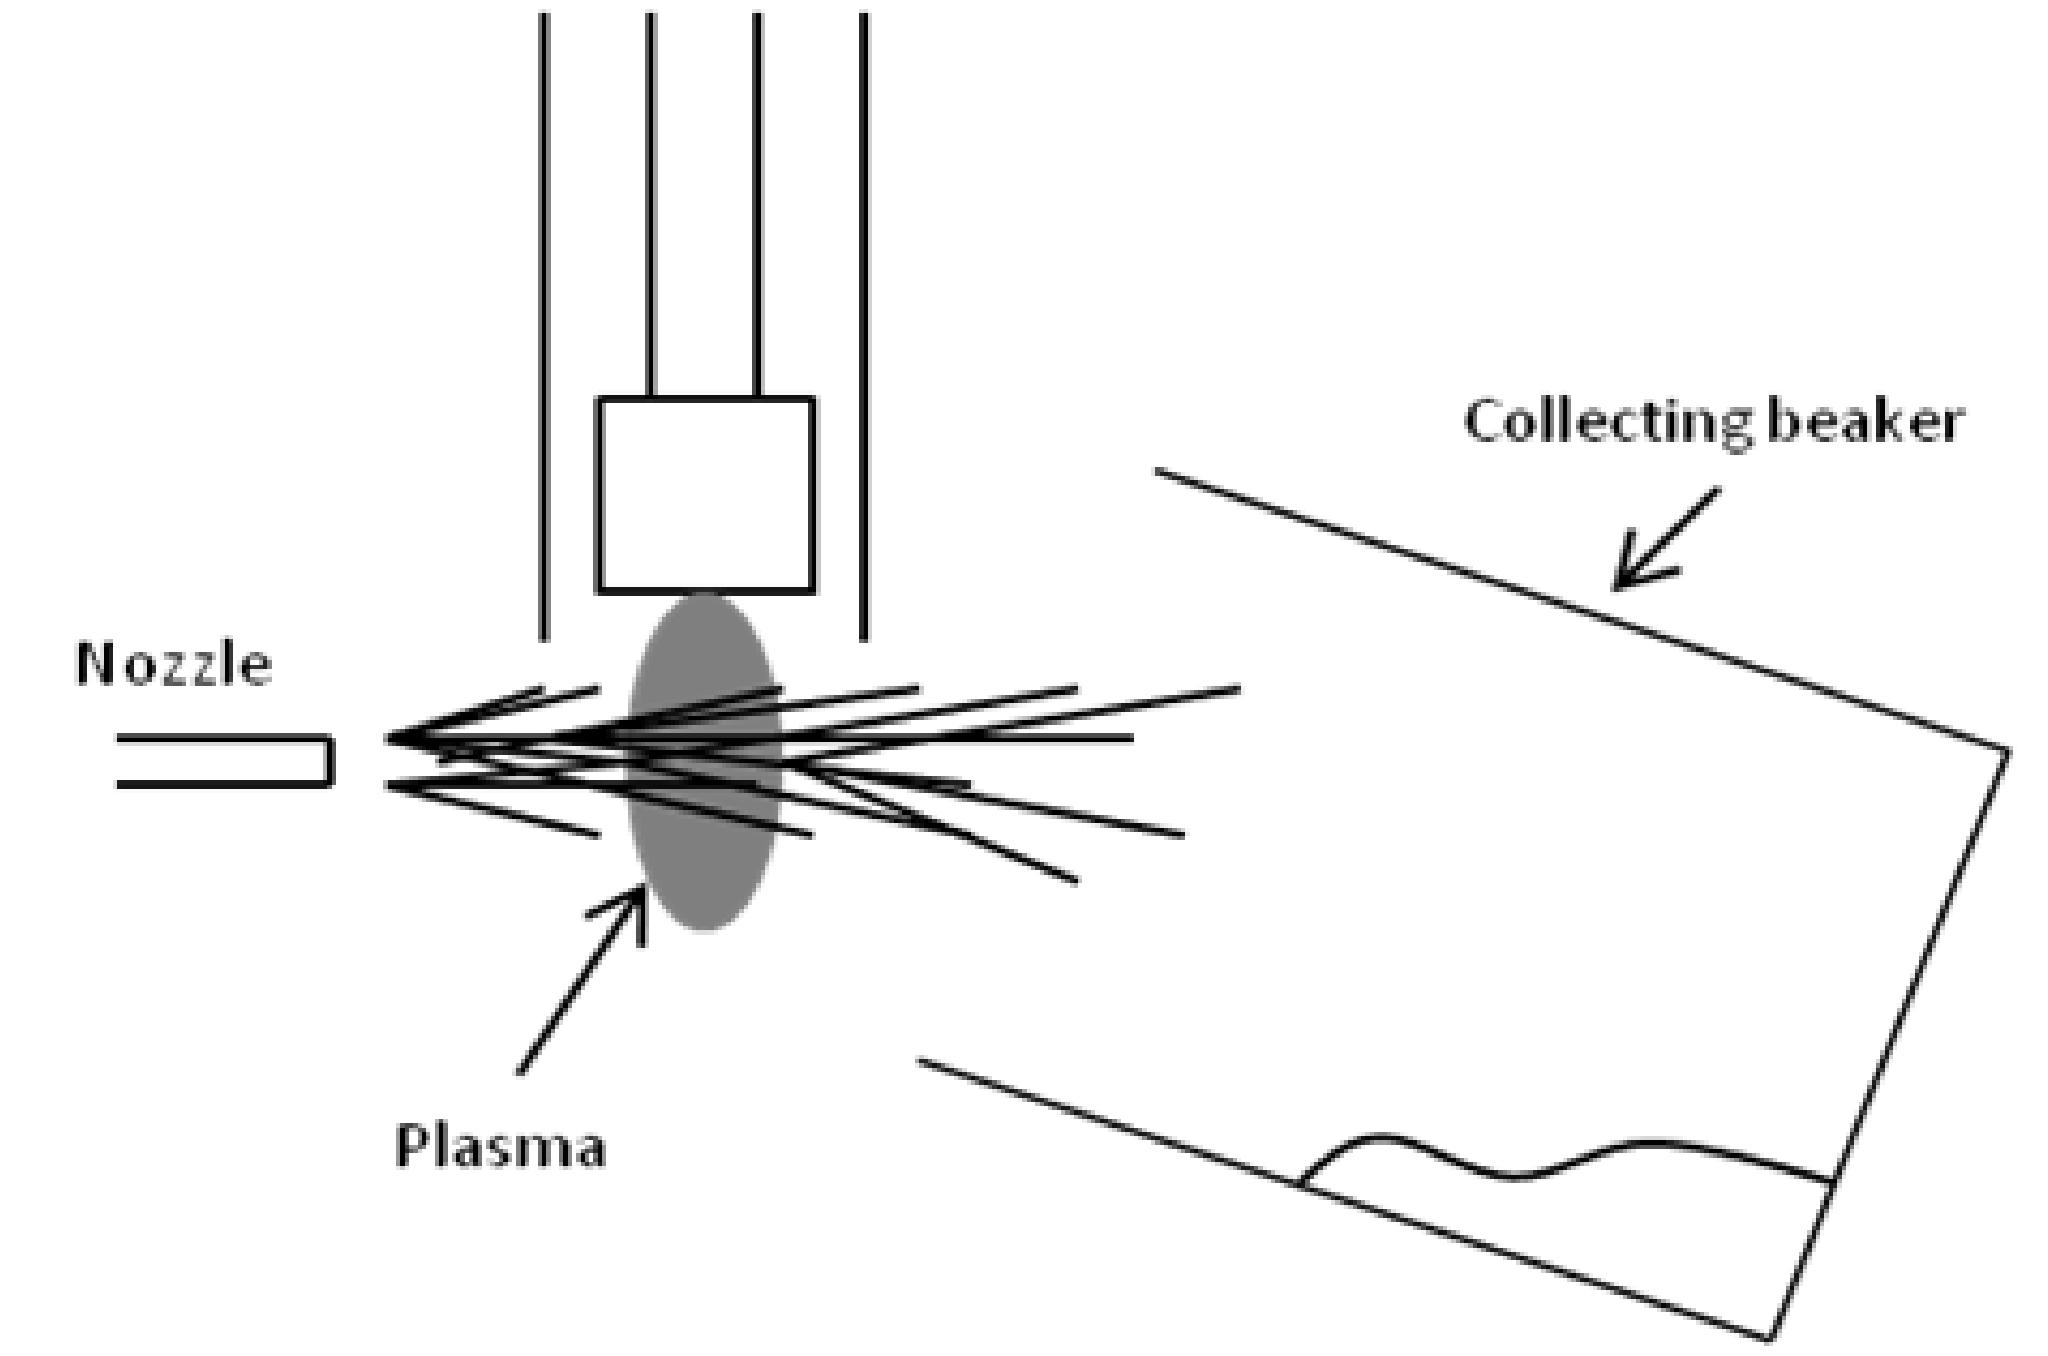
\includegraphics[width=0.9\textwidth]{Figure6_word.jpg}
  \caption{Set-up for introducing water directly into the active plasma region.  A greenhouse sprayer injects water from the side of the plasma source; water is collected in a beaker on the other side}
  \label{fig:spray_scheme}
\end{figure}

A comparison of batch and greenhouse sprayer configurations for generation of nitrate in solution per unit energy is shown in \cref{fig:nitro_compare_power}. It is found that in general the greenhouse sprayer configuration performs more favorably than the batch treatment design. This is especially clear at higher powers. Moreover, the performance of the greenhouse sprayer configuration appears to improve with increasing power delivered to the plasma. However, increasing plasma power also has some negative effects. One is an increased rate of erosion of the powered electrode. A second negative consequence is poorer matching of the load impedance resulting in increased reflected power back to the generator. Both of these effects decrease the lifetime of the design; decreasing the lifetime of the generator is particularly undesirable because of its cost.

Another issue with the greenhouse sprayer configuration that ultimately curtails further investigation is the instability of the plasma. The sprayer must be placed such that droplets do not touch the surface of the powered electrode or else the plasma is immediately extinguished. Moreoever, even if the sprayer is properly placed and the electrode is not wetted, the plasma actively trys to avoid the droplet stream. Typically even in the most optimized sprayer set-up, the plasma extinguishes after a few tens of seconds. Compare this with the batch set-up in which water can be treated continuously for multiple hours.

\subsection{Built-in Nozzle}

\begin{figure}[htbp]
  \centering
  \includegraphics{nozzle_diagram.png}
  \caption{Schematic of the nozzle electrode spray-through configuration}
  \label{fig:nozzle}
\end{figure}

\Cref{fig:nozzle} shows a schematic of the nozzle electrode experimental design. In terms of plasma-liquid contact, the concept is very similar to \cref{fig:spray_scheme} except the droplets are introduced vertically through the VHF source's inner conductor. Unfortunately, the nozzle electrode design suffers from the same pitfall as the greenhouse sprayer design. During operation, the plasma actively avoids the water droplets, moving with the cyclonic flow of the gas feed around the outside of the droplet stream. It is speculated that the droplet stream may form a Faraday cage inhibiting the discharge. Additionally, the surface non-uniformity introduced by the nozzle on the electrode leads to faster surface erosion.

\section{Base electrode designs}
\label{sec:electrodes}

As mentioned in \cref{sec:spray_bottle}, plasma erosion of the source's powered electrode can occur, especially at higher powers. Evidence of this erosion can be seen both with the naked eye (see \cref{fig:alum_damage_full}) and in the optical emission spectrum of the discharge. \Cref{fig:OES_alum_damage} shows the presence of an atomic aluminum line at 395 nm and several AlO bands between 425 and 575 nm. Visually, this emission manifests itself as an intense bright blue; an example of it can be seen in \cref{fig:diox_argon}.

\begin{figure}[htbp]
  \centering
  \includegraphics{damaged_aluminum_OES_spectrum.png}
  \caption{OES spectrum of plasma damaged aluminum electrode}
  \label{fig:OES_alum_damage}
\end{figure}

\begin{figure}[htbp]
  \centering
  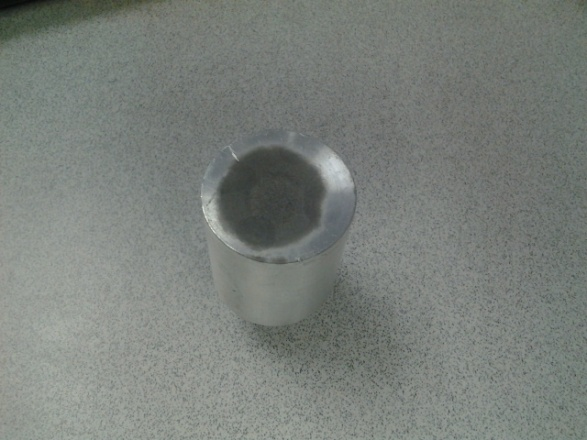
\includegraphics{full_size_alum_electrode_damage.jpg}
  \caption{Image of aluminum electrode after plasma erosion}
  \label{fig:alum_damage_full}
\end{figure}

The plasma damage to the electrode can be investigated more closely using Secondary Electron Microscopy (SEM) and Energy Dispersive X-ray Spectroscopy (EDS). Even with a 1mm zoom (\cref{fig:alum_damage_1mm}), the growth of a damage layer is evident. Taking an EDS measurement of the clean aluminum yields the spectrum shown in \cref{fig:EDS_clean_alum}. Unsurprisingly, the spectrum shows almost pure aluminum with a trace of magnesium. An EDS scan of the damaged aluminum portion, however, reveals the growth of substantial carbon and oxygen peaks (\cref{fig:EDS_damaged_alum}). The oxidation is unsurprising considering the flow gas is often compressed air and the ambient environment is also air (also consistent with the OES spectrum (\cref{fig:OES_alum_damage})). The carbon could be coming from oils/hydrocarbons present in the compressed air feed.

\begin{figure}[htbp]
  \centering
  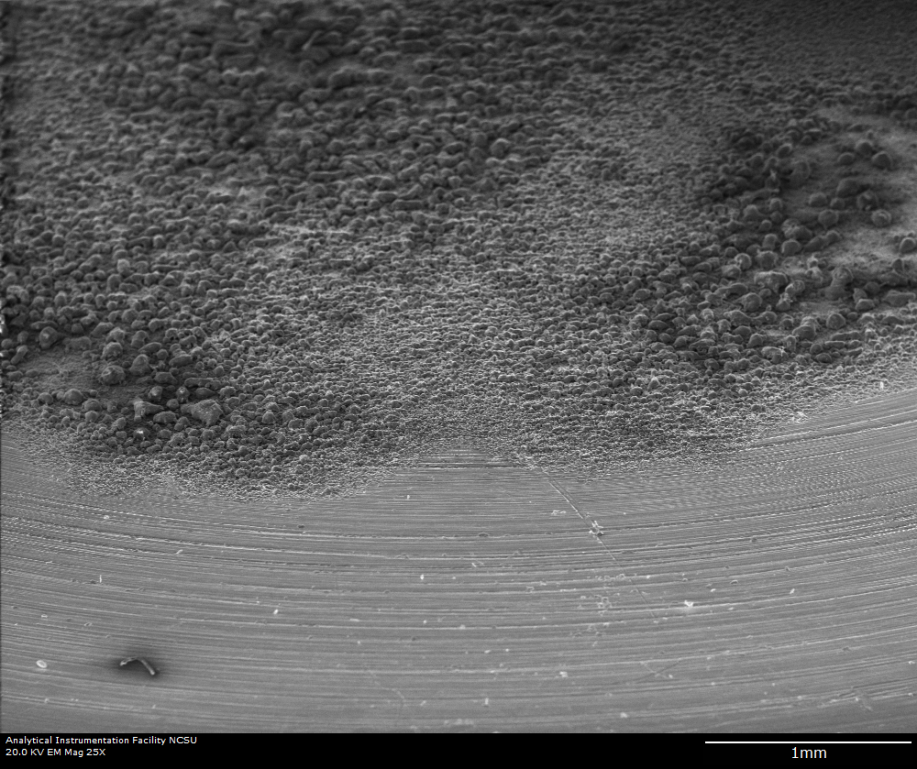
\includegraphics{1mm_zoom_tilt_alum_electrode_damage.png}
  \caption{SEM image of aluminum electrode after plasma erosion. 1mm zoom. 45 degree tilt.}
  \label{fig:alum_damage_1mm}
\end{figure}

\begin{figure}[htbp]
  \centering
  \includegraphics[width=0.9\textwidth, height=0.9\textheight, keepaspectratio]{clean_alum_eds.png}
  \caption{Energy dispersive X-ray spec (EDS) for clean aluminum electrode}
  \label{fig:EDS_clean_alum}
\end{figure}

\begin{figure}[htbp]
  \centering
  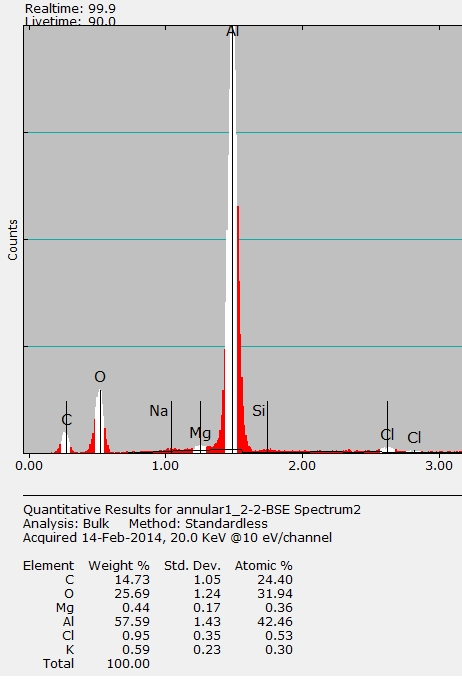
\includegraphics[width=0.9\textwidth, height=0.9\textheight, keepaspectratio]{damaged_alum_eds.png}
  \caption{Energy dispersive X-ray spec (EDS) for plasma eroded aluminum electrode}
  \label{fig:EDS_damaged_alum}
\end{figure}

In an attempt to prolong the lifetime of the powered electrode, metals other than aluminum are considered. A relatively inexpensive choice is brass. Overall, brass performs much better than aluminum. Between 300-700 W, there is no plasma-metal interactions observed with OES or presence of pitting when the plasma is turned off. Typically aluminum begins to erode around 560 W. When the brass electrode is run between 700-1000 W, plasma-metal interactions are evinced by a plasma color change as well as an increase in the intensity of the emitted light. A comparison of the plasma OES with and without metal interactions is shown in \cref{fig:OES_brass_damage}. The 560 W spectrum shows a more or less normal air plasma spectrum: NO bands between 230 and 290 nm (along with their 2x peaks around 500nm) and an OH band around 310 nm. However, the 945 W spectrum is dominated by sharp copper and zinc atomic lines. Despite the presence of copper and zinc in the discharge emission, no visual damage appears on the electrode surface when operated between 700 and 1000 W. However, if the power is raised too much over 1000 W, surface pitting and scarring analagous to the damage on the aluminum electrode are observed (see \cref{fig:brass_damage_full}).

\begin{figure}[htbp]
  \centering
  \includegraphics[width=0.9\textwidth]{damaged_brass.jpg}
  \caption{Image of brass electrode after plasma erosion}
  \label{fig:brass_damage_full}
\end{figure}

\begin{figure}[htbp]
  \centering
  \includegraphics{damaged_brass_OES_spectrum.png}
  \caption{OES spectrum of plasma damaged brass electrode}
  \label{fig:OES_brass_damage}
\end{figure}

\section{Water Electrodes}
\label{sec:water_electrodes}

An ideal plasma-liquid geometry has to provide both maximum interfacial contact between reactive plasma species and the liquid phase as well as system components that are resistent to plasma corrosion. Unfortunately, none of our previous configurations realize this goal. However, by utilizing the unique nature of the VHF source and recognizing that the entire coaxial structure is DC grounded, we can do something rather novel. We can apply a liquid layer to the surface of the powered electrode without worry of causing a short circuit. With this configuration, shown in \cref{fig:water_electrode_scheme}, the treated water is exposed to the most reactive part of the plasma. Both ion and electron fluxes to the water surface are anticipated to be much higher than in the batch configuration. Additionally, powered plasma-facing solid surfaces are completely eliminated from the geometry. The liquid surface is forever renewable. This reduces system cost as well as experimental down-time.

\begin{figure}[htbp]
  \centering
  \includegraphics[width=0.9\textwidth]{water_electrode_geometry.png}
  \caption{Representative experimental set-up for using a ``water'' electrode}
  \label{fig:water_electrode_scheme}
\end{figure}

The actual design of the water electrode can be seen in \cref{fig:water_electrodes_image}. The electrode of most utility, the ``pure'' water electrode, is shown on the right. The pure water electrode has no powered metal surfaces; the powered surface is 100\% water. If some plasma-metal contact is desired, for instance if the contact favorably modifies some plasma or liquid application variable, then the ``annular'' electrode shown on the left can be used.

\begin{figure}[htbp]
  \centering
  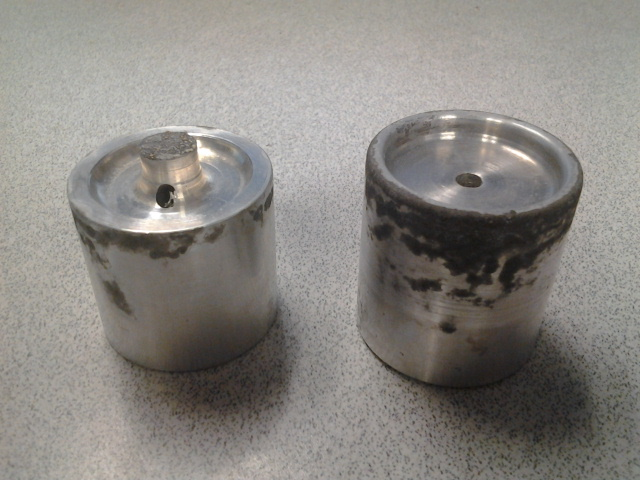
\includegraphics[width=0.9\textwidth]{water_and_annular_electrodes.jpg}
  \caption{Image of the two versions of ``water'' electrodes. The ``annular'' version still allows a small metallic area of plasma contact. In the ``pure'' version, the plasma has no metallic content with the powered electrode. The powered surface is entirely composed of water.}
  \label{fig:water_electrodes_image}
\end{figure}

\Cref{fig:annular_vs_water_oes} compares stereotypical OES spectra obtained for annular and pure water electrodes running at 700 W. Evidence of plasma-metal contact with the annular electrode is evident in the presence of aluminum atomic lines and AlO molecular bands. Additionally, there is a sodium line from sputtering of the tap water. The pure water electrode spectrum is much less intense and consists only of OH bands.

\begin{figure}[htbp]
  \centering
  \includegraphics{annular_vs_water_electrode_oes.png}
  \caption{Comparison of OES spectra for annular and pure water electrodes}
  \label{fig:annular_vs_water_oes}
\end{figure}

\Cref{fig:pow_sweep_water} shows the effect of increasing power on the optical emission spectrum with the pure water electrode. Because the plasma is in immediate contact with the water surface and not any solid surfaces, the device can be operated at much higher powers. Whereas with a metal electrode the source cannot be run at powers much greater than 700 W without significant damage to the electrode, the pure water electrode can be run up to 1155 W. The only reason that the device cannot be operated at even higher powers is because of the increased difficulty in matching impedances using the main and stub lines; reflected power becomes high enough to potentially damage the generator.

Up above 1000 W, aluminum atomic lines and AlO bands become apparent (\cref{fig:pow_sweep_water}). The presence of the aluminum associated emissions is interesting because the metal is removed from the gaseous discharge region by the few milimeter thick water layer; this probably explains why the intensities are significantly below that of discharges with direct plasma-metal contact (see \cref{fig:annular_vs_water_oes}). However, the existence of any aluminum lines at all implies that the discharge is penetrating the aqueous phase to reach the metal. This is perhaps indirect evidence of high charged particle fluxes to the water electrode surface, suggesting that the pure water electrode design is a good one for maximizing interactions between the plasma and aqueous phases.

\begin{figure}[htbp]
  \centering
  \includegraphics{water_electrode_power_sweep_oes.png}
  \caption{OES spetra showing power sweep with pure water electrode. Relatively small aluminum peaks grow in at very high powers.}
  \label{fig:pow_sweep_water}
\end{figure}

% Note that there is a lot of OH rotational measurement as well as nitrite and nitrate concentration measurements for the water electrodes that are in my ICOPS 2014 presentation. I think the data looks like a bunch of garbage with no clear trends so I'm omitting it for now. However, if I need more material, I can perhaps come back to it.

\subsection{Early Absorption Work}

\begin{figure}[htbp]
  \centering
  \includegraphics[width=\textwidth]{abs_setup.png}
  \caption{Expermental set-up for absorption spectroscopy with the water electrode.}
  \label{fig:expt_abs}
\end{figure}

\begin{figure}[htbp]
  \centering
  \includegraphics[width=\textwidth]{raw_absorption_spec.png}
  \caption{Raw optical spectra in the OH wavelength region for different plasma powers. The series ``Without plasma'' shows the light intensity of the broadband light source. The other series clearly show the absorption of light by gaseous OH radicals.}
  \label{fig:raw_abs}
\end{figure}

\begin{figure}[htbp]
  \centering
  \includegraphics[width=\textwidth]{net_absorption_spec.png}
  \caption{Net results obtained by subtracting plasma absorption spectra from broadband light source spectrum and normalizing. Obvious OH X-A transition fingerprint}
  \label{fig:net_abs}
\end{figure}

Some idea of the magnitude of OH produced by the water electrode geometry can be gained by performing absorption spectroscopy. A picture of the experimental set-up is shown in \cref{fig:expt_abs}. The diameter of the plasma column is approximately 2 cm. We pass a broadbeam light source through slits cut in the outer conductor of the VHF shource. Mirrors on each slit side are used to route the light beam through the plasma column for a total of 4 passes and a total path-length of approximately 8 cm. After completing 4 passes, the beam enters an optical fiber connected to a high resolution spectrometer. The spectrum of the broadband light source in the absence of plasma is presented as series ``no-plasma'' in \cref{fig:raw_abs}. When the plasma is turned on, there is significant attenuation of the broadband signal in the region of the OH X-A electronic transition as shown in \cref{fig:raw_abs}. The amount of attenuation appears to be insensitive to the electrical power dissipated in the plasma. Subtracting the plasma + broadband ssignal from the broadband signal and normalizing produces the plot shown in \cref{fig:net_abs}. The fingerprint of the OH X-A transition is evident.


\section{Exploring Aqueous Chemistry Generated by Plasma-Liquid Interactions}
\label{sec:aq_chem}

In addition to plasma characterization with OES, additional research has focused on optimizing and understanding generation of nitrates and nitrites in aqueous solution.  Several variables have been explored, including power supplied by the 162 MHz generator, flow rate of the feed gas, type of interface between the plasma and water phases, and the effect of aqueous impurities, particularly basic species. The majority of experiments were performed using the experimental set-up shown in \cref{fig:batch_scheme}.  However, the greenhouse sprayer scheme shown in \cref{fig:spray_scheme} was also employed.  The number of impurities and basic species in water were controlled in two manners.  The first was the choice between distilled and tap water, with the former containing negligible impurities and the latter containing impurities found in Raleigh's municipal water supply; these impurities are summarized in \cref{tab:tap_water}.  The most relevant item in \cref{tab:tap_water} is the alkalinity, which comes primarily from the carbonate system.  At a pH of 8.4, it is reasonable to assume that the tap water alkalinity is completely due to bicarbonate. \cite{benjamin2014water} Using this assumption, the concentration of bicarbonate in tap water is .50 mmol/L.  The concentration of bicarbonate can also be directly controlled by adding measured amounts of NaHCO3.   NaHCO3 can be added pre- or post-exposure depending on the experiment.  The motivation for adding basic species like NaHCO3 to solution is that they are known to react with dissolved NO and NO2 to form nitrite. \cite{greenwood1984chemistry} Thus basic species concentrations can be a control knob for adjusting the nitrogen chemistry in PAW.

\begin{table}[htpb]
  \begin{center}
    \begin{tabular}{|c |c |}
      \hline
      pH & 8.4 \\\hline
      Free CO$_2$ & .23 \\\hline
      Total alkalinity (mg/L as CaCO$_3$) & 24.8 \\\hline
      Total hardness (mg/L as CaCO$_3$) & 24.4 \\\hline
      Total dissolved solids (mg/L) & 150 \\\hline
      Specific conductivity ($\mu$S/cm) & 225 \\\hline
      Iron (mg/L) & .01 \\\hline
      Manganese (mg/L) & .02 \\\hline
      Fluoride (mg/L) & .78 \\\hline
      Chloride (mg/L) & 13.3 \\\hline
      Silica (mg/L) & 8.12 \\\hline
      Silt density index (SDI) & 5.00 \\
      \hline
    \end{tabular}
  \end{center}
  \caption{Impurities in Raleigh tap water}
  \label{tab:tap_water}
\end{table}

At a gas flow rate of .14 m3/min, an exposure time of 3 minutes, and a treatment volume of 150 mL distilled water, nitrate concentrations were determined for powers ranging from 385 to 630 W and are shown in \cref{fig:nitrogen_vs_energy}.  For a better comparison with spray treatment results shown in \cref{fig:nitrogen_vs_energy_spray}, the horizontal axis is defined in terms of the energy deposited in the plasma per mass of water exposed to the plasma.  The results indicate a general downward trend in nitrate concentration with respect to power and total energy deposition.   To decouple the effects of power and total energy deposition, a second experiment was conducted in which treatment times were varied with power in order to keep the total energy delivered to the plasma constant.  Consequently, whereas the exposure time was 3 minutes for a 420 W plasma, exposure time was only 2 minutes for a 630 W plasma for a constant plasma energy deposition of 75.6 kJ; for comparison with figure 17, the energy deposited in the plasma per mass of exposed water was 504 kJ/kg.  Gas flow was again .14 m3/min and water volumes were 150 mL.  Results from the second experiment are shown in \cref{fig:nitrogen_vs_power}.  Though the plasma energy deposition is constant, nitrate concentrations in both tap and distilled water samples decrease with increasing power, consistent with the trend in figure 17.  Though no nitrite appears in distilled water samples, nitrite concentrations increase in tap water with increasing power.  The total nitrogen anion levels in tap and distilled water samples are within experimental error for powers between 420 and 560 W.

\begin{figure}[htbp]
  \centering
  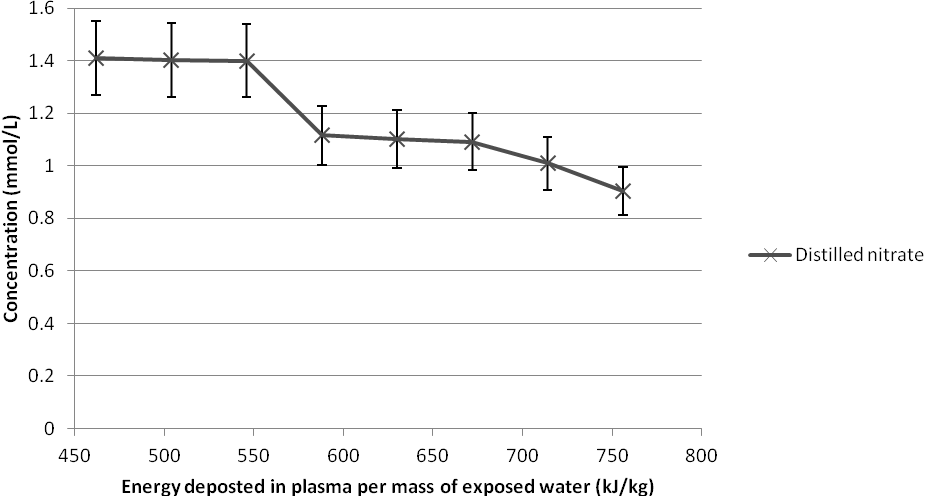
\includegraphics{Figure17_word.png}
  \caption{Nitrate concentration in distilled water versus energy deposited in the plasma per mass of exposed water. No detectable amount of nitrite generated}
  \label{fig:nitrogen_vs_energy}
\end{figure}

\begin{figure}[htbp]
  \centering
  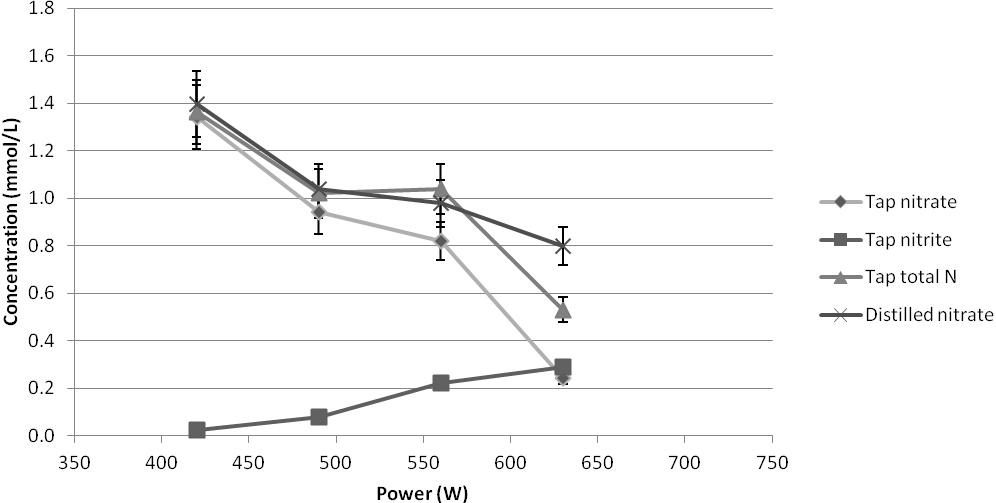
\includegraphics{Figure18_word.png}
  \caption{Nitrate and nitrite concentrations in tap water versus power.  Treatment times scaled such that for each power setting, total energy deposited in system is constant at 504 kJ/kg H2O}
  \label{fig:nitrogen_vs_power}
\end{figure}

Another variable explored was gas flow rate.  For an exposure of 3 minutes, a treatment volume of 150 mL distilled water, and a plasma power input of 420 W, nitrate concentrations were measured for flow rates of .08, .11, and .14 m3/min and are recorded in \cref{fig:nitrogen_vs_flow}.  A factor of 4.9 improvement in nitrate concentration is observed between .08 and .14 m3/min flow settings.  Again no detectable amount of nitrite was observed.

\begin{figure}[htbp]
  \centering
  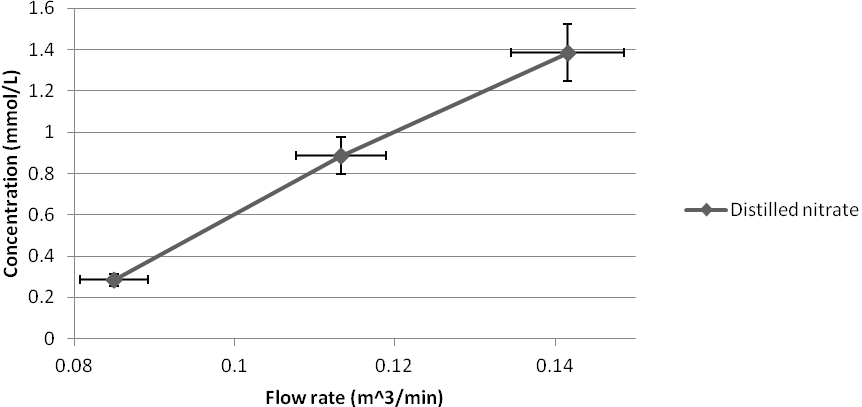
\includegraphics{Figure19_word.png}
  \caption{Nitrate concentration in distilled water versus air flow rate. No detectable amount of nitrite generated}
  \label{fig:nitrogen_vs_flow}
\end{figure}

One variable with remarkable effects on nitrogen species concentration is the presence of basic species before plasma exposure and also addition of basic species after plasma exposure.  As mentioned in the experimental section and as will be touched on further in the discussion section, basic species are known to react with dissolved NO and NO2 (which are formed in the plasma) to form nitrite. \cref{tab:bicarb} summarizes a series of experiments in which the effect of adding approximately 6 mmol/L of sodium bicarbonate before or after plasma exposure was observed on tap and distilled water substrates (200 mL volume).  In both distilled and tap water samples, adding sodium bicarbonate before plasma exposure produced significantly more nitrite than when it was added post-exposure, which in turn produced significantly more nitrite than when no bicarbonate was added at all.  For all three treatment schemes, tap water ended with more nitrite than distilled.  Nitrate trends were not as clear.

\begin{table}[htpb]
  \begin{center}
    \begin{tabularx}{\textwidth}{|c |c |c |X |c |}
      \hline
      \textbf{Nitrite (mmol/L)} & \textbf{Nitrate (mmol/L)} & \textbf{pH} & \textbf{Description} & \textbf{Sample reference \#} \\\hline
      .041 & 1.09 & 3.18 & Tap, no NaHCO3 addition & 1 \\\hline
      2.43 & .795 & 7.99 & Tap, 5.71 mmol/L NaHCO3 added pre-exposure & 2 \\\hline
      .617 & .981 & 7.68 & Tap, 6.19 mmol/L NaHCO3 add post-exposure & 3 \\\hline
      .004 & .795 & 2.88 & Distilled, no NaHCO3 addition & 4 \\\hline
      .854 & .273 & 8.02 & Distilled, 5.71 mmol/L NaHCO3 added pre-exposure & 5 \\\hline
      .235 & 1.37 & 7.55 & Distilled, 6.67 mmol/L NaHCO3 added post-exposure & 6 \\\hline
    \end{tabularx}
  \end{center}
  \caption{Dependence of nitrogen ionic species on water type and amount of NaHCO3 in solution.  The sample \#'s are used as references in the discussion section}
  \label{tab:bicarb}
\end{table}

Another variable that was manipulated was the time between plasma exposure and post-exposure addition of NaHCO3. \Cref{fig:nitrogen_vs_time_delay} shows that while the total molar concentration of ionic nitrogen species is a constant, increasing the time between plasma exposure and NaHCO3 addition increases nitrate concentration and decreases nitrite concentration.

\begin{figure}[htbp]
  \centering
  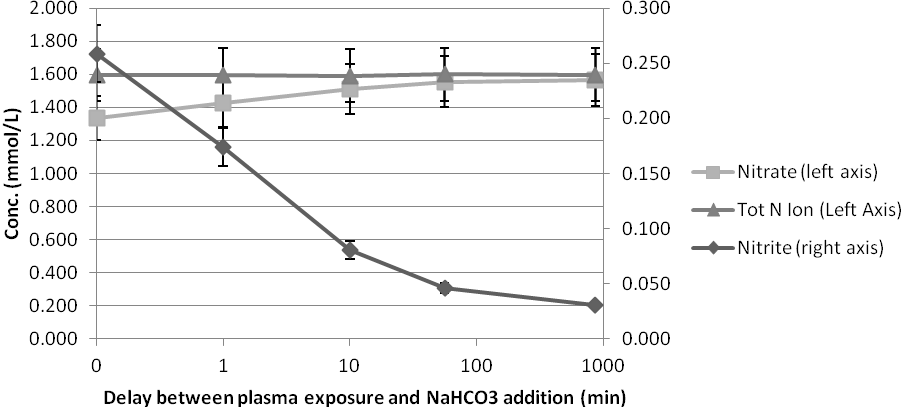
\includegraphics{Figure20_word.png}
  \caption{Effect of time delay between plasma exposure and bicarbonate addition on nitrite and nitrate species concentrations}
  \label{fig:nitrogen_vs_time_delay}
\end{figure}

A fundamental change in the set-up of the system can be realized by removing the stagnant water volume from underneath the electrode and instead spraying the water substrate directly through the active plasma region as described in the experimental section and as shown in \cref{fig:spray_scheme}.  Some difficulty is experienced in maintaining the plasma during water spray operation.  The plasma actively attempts to avoid the region through which the water passes; if the water spray blankets the entire area which the plasma normally occupies, the discharge may extinguish.  However, if the plasma is maintained, the increased biphasic interaction is demonstrated by frequent orange light emission from excited sodium in tap water.  For this alternative geometry the effects of power and gas flow rate on nitrate uptake are in opposition to the trends witnessed for the stationary water phase geometry.   For one pass of distilled water through the active plasma region \cref{fig:nitrogen_vs_energy_spray} shows increasing nitrate uptake with increasing power for a gas flow rate of .11 m3/min (no nitrite formed).  Instead of power on the x-axis, energy per kg of exposed water is used in order to enable a comparison to the results shown in \cref{fig:nitrogen_vs_energy}.  The concentration of nitrate generated in the water is an order of magnitude less in \cref{fig:nitrogen_vs_energy_spray} than it is in \cref{fig:nitrogen_vs_energy}, but the energy usage per kg of exposed water is also an order of magnitude less.  A more obvious comparison between spray and batch treatments can be done by combining \cref{fig:nitrogen_vs_energy,fig:nitrogen_vs_energy_spray} and plotting the amount of nitrate generated per energy usage as a function of power, as is done in \cref{fig:nitro_compare_power}.  The most efficient nitrate generation occurs at 700 W using spray treatment, yielding 4.6 μmols of nitrate per kJ.  However, based on the observed trends, even more efficient nitrate generation may be realized by continuing to increase power with spray treatment or by decreasing power with batch treatment.  \Cref{fig:nitro_vs_flow_spray} shows that spray treatment efficiency may also be improved by decreasing gas flow rate.

\begin{figure}[htbp]
  \centering
  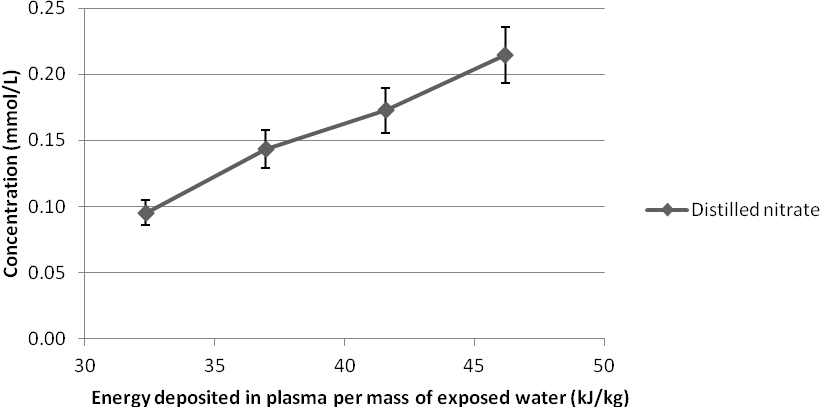
\includegraphics{Figure21_word.png}
  \caption{Dependence of nitrate uptake on plasma energy deposition for water sprayed through the active plasma region.  Compare with results in Figure 17 for batch treatment}
  \label{fig:nitrogen_vs_energy_spray}
\end{figure}

\begin{figure}[htbp]
  \centering
  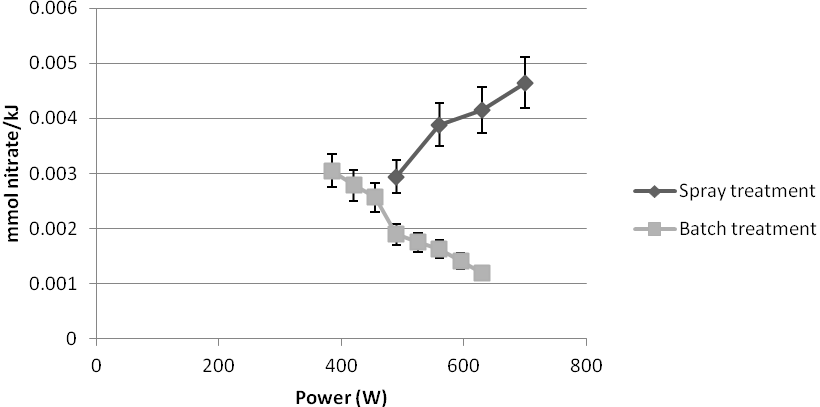
\includegraphics{Figure22_word.png}
  \caption{Comparison between batch and spray treatment methods using mmol of nitrate generated per kJ of electrical energy as the figure of merit.  For lower powers batch treatment is more energetically efficient for nitrate generation.  For higher powers spray treatment is more efficient.  Further investigation of batch process at lower powers and spray process at higher powers required to determine optimal process for nitrate generation}
  \label{fig:nitro_compare_power}
\end{figure}

\begin{figure}[htbp]
  \centering
  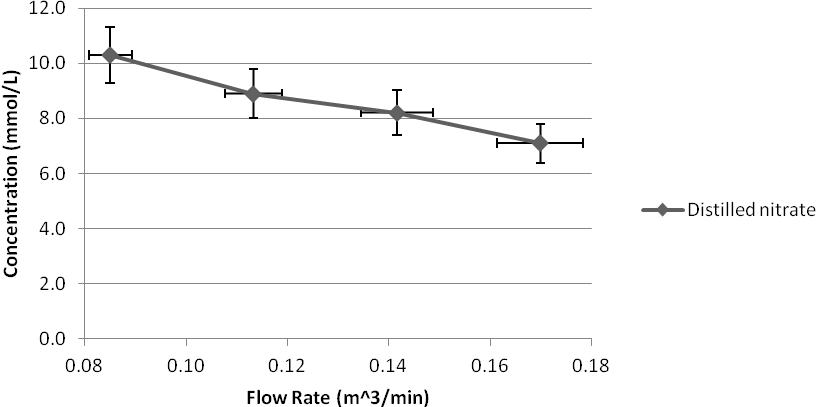
\includegraphics{Figure23_word.png}
  \caption{Dependence of nitrate uptake on gas flow rate for water sprayed through the active plasma region. Power = 560 W.}
  \label{fig:nitro_vs_flow_spray}
\end{figure}

The species concentration trends observed in \cref{fig:nitrogen_vs_energy,fig:nitrogen_vs_power,fig:nitrogen_vs_energy_spray} are believed to result from the dependence of electron density and gas temperature on delivered power and from the dependence of interfacial mass transfer on system configuration.   Consider the trend shown in \cref{fig:nitrogen_vs_energy,fig:nitrogen_vs_power} for the concentration of nitrate as a function of power and energy deposition for the case where the water surface is held stationary directly under the plasma.  As power increases, the amount of nitrate produced decreases.  It is possible that the increase in electron density that occurs simultaneously with increasing power creates a more reductive environment which enables more formation of  nitrite as evidenced in \cref{fig:nitrogen_vs_power} (oxidation state = +3) or other more reduced NOx forms such as NO (+2), NO2 (+4), and N2O (+1)  relative to nitrate (+5).  This analysis, however, is confounded by the trend observed in \cref{fig:nitrogen_vs_energy_spray} in which nitrate uptake increases with increasing power when water is sprayed through the active plasma region.  A tentative explanation is that when the water surface is held stationary below the plasma the outgoing convective flow of the feed gas restricts diffusion of water vapor into the plasma region, a restriction that is not present when water is directly injected into the discharge.  If water vapor is present in the active plasma region, an increase in power should correspond to an increase in hydroxyl radical formation because of an increase in the rate of electron-impact dissociation.  This should increase the oxidizing nature of the plasma and subsequently increase nitrate production; this is observed in \cref{fig:nitrogen_vs_energy_spray} for direct water injection.  While this logic may also extend to the case where the plasma hovers over the stationary water surface, it can be expected to occur to a much more limited degree compared to the direct injection case because the convective wind of the feed gas whisks water vapor away from the active plasma region.  Consequently there is not a sufficiently large increase in the oxidizing character of the plasma to offset the increase in reductive character due to electron density; the nitrate concentration then decreases with power as observed in \cref{fig:nitrogen_vs_energy,fig:nitrogen_vs_power}.

The argument presented in the previous paragraph also supports the trend shown in \cref{fig:nitro_vs_flow_spray}, where nitrate concentration decreases with increasing gas flow rate for the case of direct water injection.  An increase in gas flow rate decreases the residence time of gas molecules in the glow region, decreasing the gas temperature.  Decreasing gas temperature decreases the vaporization rate of liquid droplets, leading to a decreased concentration of hydroxyl in the plasma and a decreased ability to oxidize gaseous nitrogen species to nitrate.  This theory, however, contradicts the trend seen in \cref{fig:nitrogen_vs_flow} for stationary water where nitrate increases with flow rate.  One explanation is that the decreased transit time between plasma and water phases results in a decreased radical species recombination rate capable of offsetting the proposed decrease in hydroxyl concentration in the plasma region.

In addition to arguing that increasing hydroxyl concentration in the plasma region should increase the oxidizing nature of the discharge and subsequently increase nitrate concentrations, a stoichiometric outlook suggests that introducing another source of elemental oxygen increases the ratio of oxygen to nitrogen in the discharge, allowing greater formation of high O:N ratio species like NO$_3^-$.  This theory could be explored more in future experiments with varying feed ratios of N$_2$ and O$_2$.

\begin{figure}[htbp]
  \centering
  \includegraphics{H2O2_measurement.png}
  \caption{Hydrogen peroxide concentration in solution as a function of plasma power}
  \label{fig:H2O2}
\end{figure}

In order to address the last variable considered in the study, the effect of basic aqueous species on nitrogen ion concentrations, it is worthwhile to summarize some of the potentially important reaction mechanisms involving reactive nitrogen and oxygen species in solution.   Aside from nitrite and nitrate ions, hydrogen peroxide is known to be a prevailing species in solution following plasma treatment \cite{traylor2011long}; this is confirmed by colorimetric analysis in \cref{fig:H2O2}.  Moreover, volatile NO$_x$ species like NO and NO$_2$ may also be present and may be responsible for the observation in \cite{traylor2011long} of a spectroscopic peak at 262 nm when samples are sealed; when samples are left unsealed, the 262 nm peak is not observed.  Relevant redox reactions involving these species are taken from \cite{brisset2012peroxynitrite}  and \cite{greenwood1984chemistry} and presented in Table 7.

\begin{table}[htpb]
  \begin{center}
    \begin{tabular}{|l |c |}
      \hline
      \textbf{Reaction Description} & \textbf{Reaction reference \#} \\\hline
      $4NO + O_2 + 2H_2O \rightarrow 4H^+ + 4NO_2^-$ & 1 \\\hline
      $H_2O_2 + NO_2^- \rightarrow ONOO^- + H_2O$ & 2 \\\hline
      $ONOOH \rightarrow H^+ + NO_3^-$ & 3 \\\hline
      $3HNO_2 \rightarrow 2NO + NO_3^- + H^+ + H_2O$ & 4 \\\hline
      $NO + NO_2 + 2A^- + H_2O \rightarrow 2NO_2^- + 2HA$ & 5 \\\hline
      $2NO + O_2 \rightarrow NO_2$ & 6 \\\hline
      $3NO_2 + H_2O \rightarrow 2H^+ + 2NO_3^- + NO$ & 7 \\\hline
      $4NO_2\,(or\,2N_2O_4) + O_2 + 2H_2O \rightarrow 4HNO_3$ & 8 \\\hline
    \end{tabular}
  \end{center}
  \caption{Important reactions between nitrogen and oxygen species which may occur in the aqueous phase}
  \label{tab:reactions}
\end{table}

References \cite{greenwood1984chemistry} and \cite{Lukes2014b} illustrate that peroxynitrous acid (ONOOH) is formed as an unstable intermediate during the oxidation of acidified aqueous solutions of nitrites to nitrates using H$_2$O$_2$, and that such solutions are more highly oxidizing than either H$_2$O$_2$ or HNO$_2$ alone.  Because the conditions of the former statement are satisfied in PAW, it is reasonable to assume that peroxynitrous acid is the intermediate species between nitrite and nitrate as hypothesized in \cite{traylor2011long}.  Moreover, the much greater efficacy of PAW compared to a control mixture of nitric acid and hydrogen peroxide for degrading bacteria \cite{burlica2010bacteria} further suggests the presence of a reactive oxidizing species like peroxynitrous acid.

Applying the equations in \cref{tab:reactions} to the investigation of basic species effects on nitrogen ion formation provides some insight into observed trends in \cref{fig:nitrogen_vs_time_delay}, where the nitrite and nitrate molar concentrations in PAW as a function of time delay between plasma exposure and addition of sodium bicarbonate are shown.  The +3 oxidation state of nitrogen in water, e.g. nitrite/nitrous acid, is unstable at acidic pH.  Following plasma exposure, PAW is acidic and reaction (4) in \cref{tab:reactions} will occur as long as the solution is acidic.  Subsequently, for long time delays between exposure and base addition, the solution has time to convert nearly all aqueous nitrogen species into nitrate.  If base is added immediately following exposure more nitrite will be preserved in solution.  Moreover, if base is added while +2 and +4 oxidation state nitrogen is present in solution, e.g. species such as NO and NO$_2$, reaction (5) may occur.  It is conceivable that reaction (5) is responsible for the nitrite trends witnessed in \cref{tab:bicarb}.  Tap water contains more basic species than distilled water which theoretically contains none other than a 10-7 molar concentration of hydroxide.  Subsequently, tap water contains more A- species that are capable of reacting with NO and NO2 to form nitrite.  Moreover, if a large quantity of additional base is added to solution before plasma exposure, the amount of A- available for reaction (5) increases significantly, leading perhaps to the comparatively large concentration of nitrite observed in sample 2 in Table 6.  This result is not observed to the same degree in the distilled water sample, sample 5, but some effect is still present.  Relative to solutions that received no additions, the increased presence of nitrite following post-treatment basic additions could be a combination of both reaction (4) and (5) effects, with (5) occurring when base is added quickly enough that NO and NO2 are still dissolved in solution.

Much of the theory suggested above needs to be validated by further experiment and by computational models.  Models should include the relevant chemical reactions shown in \cite{moussa2005acidity}, \cite{brisset2012peroxynitrite}, and \cite{greenwood1984chemistry} and must be coupled to reactions and mass transfer from the plasma phase. With the construction of the models in \cref{chap:basic_science} and the flexbility of the code in \cref{chap:zapdos}, exploration of solution chemistry and the theories presented here are well within reach and are on the agenda for future research.

\section{Summary}

\Cref{chap:expt_opt} describes our experimental designs for investigating plasma-liquid interactions. \Cref{sec:base} describes the base configuration where the 162 MHz plasma source is pointed downward into a reservoir of water. \Cref{sec:spray} examines trying to increase the surface area of plasma-liquid interaction by directly introducing water droplets into the plasma dischare. In \cref{sec:electrodes} we discuss the electrodes placed on the end of the VHF source's inner conductor and their tendency for plasma erosion. To increase fluxes of charged plasma species to the water surface and to alleviate electrode damage, we introduce in \cref{sec:water_electrodes} an experimental configuration in which the source is pointed upwards and water is pumped through the inner conductor to form a liquid layer on top of the powered electrode. Finally, in \cref{sec:aq_chem} we measure different aqueous specie concentrations as a function of different system variables and speculate on the observed trends. The need to extend the models presented in \cref{chap:basic_science} to confirm some of the hypotheses in \cref{sec:aq_chem} is noted. Having built and characterized these experimental configurations, it is worthwhile to explore some of the applications of plasma-liquid systems. In \cref{chap:applications} we explore a couple of these applications, including fertilization of plants using plasma activated water and degradation of persistent aqueous contaminants.
